% ============================================================
%  DISCOVERY CURRICULUM — Journey 4, Module 2
%  "The Integral Theorems"
%  Compile with: pdflatex J4_M2.tex  (run twice)
% ============================================================
\documentclass[12pt,a4paper]{article}
\usepackage[a4paper,top=2.5cm,bottom=2.5cm,left=2.8cm,right=2.8cm,headheight=15pt]{geometry}
\usepackage{amsmath,amssymb,amsthm}
\usepackage{xcolor}
\usepackage{mdframed}
\usepackage{enumitem}
\usepackage{tikz}
\usetikzlibrary{arrows.meta,calc}
\usepackage{pgfplots}
\pgfplotsset{compat=1.18}
\usepackage{booktabs}
\usepackage{fancyhdr}
\usepackage{titlesec}
\usepackage{parskip}
\usepackage{hyperref}
\hypersetup{colorlinks=true,linkcolor=NavyBlue,urlcolor=NavyBlue}

\definecolor{NavyBlue}{HTML}{1A3A5C}
\definecolor{MidBlue}{HTML}{2E6DA4}
\definecolor{Gold}{HTML}{C8922A}
\definecolor{LightBlue}{HTML}{EBF2FA}
\definecolor{LightGold}{HTML}{FDF4E3}
\definecolor{DarkGrey}{HTML}{3A3A3A}
\definecolor{BoxGreen}{HTML}{E8F5E9}
\definecolor{SidebarGrey}{HTML}{F5F5F5}

\titleformat{\section}{\Large\bfseries\color{NavyBlue}}{}{0em}{}[{\color{MidBlue}\vspace{2pt}\rule{\linewidth}{1.5pt}}]
\titleformat{\subsection}{\large\bfseries\color{MidBlue}}{}{0em}{}

\pagestyle{fancy}\fancyhf{}
\fancyhead[L]{\small\color{DarkGrey}\textit{Discovery Curriculum}}
\fancyhead[R]{\small\color{DarkGrey}\textit{Journey 4 $\cdot$ Module 2}}
\fancyfoot[C]{\small\color{MidBlue}\thepage}
\renewcommand{\headrulewidth}{0.4pt}

\newmdenv[backgroundcolor=NavyBlue!7,linecolor=NavyBlue,linewidth=2pt,leftline=true,rightline=false,topline=false,bottomline=false,innerleftmargin=14pt,innerrightmargin=10pt,innertopmargin=10pt,innerbottommargin=10pt,skipabove=14pt,skipbelow=10pt]{puzzlebox}
\newmdenv[backgroundcolor=LightGold,linecolor=Gold,linewidth=2pt,leftline=true,rightline=false,topline=false,bottomline=false,innerleftmargin=14pt,innerrightmargin=10pt,innertopmargin=10pt,innerbottommargin=10pt,skipabove=14pt,skipbelow=10pt]{discoverybox}
\newmdenv[backgroundcolor=LightBlue,linecolor=MidBlue,linewidth=1.5pt,roundcorner=4pt,innerleftmargin=14pt,innerrightmargin=10pt,innertopmargin=10pt,innerbottommargin=10pt,skipabove=14pt,skipbelow=10pt]{namebox}
\newmdenv[backgroundcolor=BoxGreen,linecolor=DarkGrey!35,linewidth=1pt,roundcorner=4pt,innerleftmargin=14pt,innerrightmargin=10pt,innertopmargin=10pt,innerbottommargin=10pt,skipabove=14pt,skipbelow=10pt]{reflectionbox}
\newmdenv[backgroundcolor=SidebarGrey,linecolor=Gold,linewidth=1.2pt,leftline=true,rightline=false,topline=false,bottomline=false,innerleftmargin=12pt,innerrightmargin=10pt,innertopmargin=7pt,innerbottommargin=7pt,skipabove=10pt,skipbelow=10pt]{thought}

\newcounter{problem}
\newenvironment{problem}[1][]{\refstepcounter{problem}\par\vspace{6pt}\noindent\textbf{\color{MidBlue}Problem \theproblem}\ifx&#1&\else\ \textit{(#1)}\fi\textbf{.}\enskip}{\par\vspace{4pt}}
\newcounter{deepproblem}
\newenvironment{deepproblem}[1][]{\refstepcounter{deepproblem}\par\vspace{6pt}\noindent\textbf{\color{NavyBlue}$\bigstar$\ Deep Problem \thedeepproblem}\ifx&#1&\else\ \textit{(#1)}\fi\textbf{.}\enskip}{\par\vspace{4pt}}

\begin{document}

\thispagestyle{empty}
\begin{center}
{\small\color{MidBlue}\textbf{DISCOVERY CURRICULUM}\quad$\cdot$\quad\textbf{JOURNEY 4: FIELDS AND SPACE}}
\vspace{0.6cm}

{\color{NavyBlue}\rule{\linewidth}{2pt}}\vspace{0.5cm}

{\Huge\bfseries\color{NavyBlue}Module 2}\\[0.3cm]
{\LARGE\bfseries\color{MidBlue}The Integral Theorems}\\[0.4cm]
{\color{Gold}\rule{0.4\linewidth}{1.2pt}}\\[0.4cm]
{\large\itshape\color{DarkGrey}
Gauss, Green, Stokes: three theorems, one idea.\\[0.15cm]
What happens inside is determined by the boundary.}

\vspace{1cm}
\begin{tabular}{rl}
\color{DarkGrey}\textbf{Journey}         & Journey 4 --- Fields and Space \\[4pt]
\color{DarkGrey}\textbf{Module}          & 2 of 6 \\[4pt]
\color{DarkGrey}\textbf{Prerequisites}   & J4 Module 1; J2 Modules 3, 6 \\[4pt]
\color{DarkGrey}\textbf{You will discover} & Gauss's divergence theorem, Stokes' theorem, Green's theorems, physical applications \\[4pt]
\color{DarkGrey}\textbf{Format}          & 7 problems $+$ 3 deep problems $\approx$ 13 pages \\
\end{tabular}
\vspace{1cm}

{\color{NavyBlue}\rule{\linewidth}{2pt}}
\end{center}

\vspace{0.5cm}
\noindent\textbf{The great unification.}
The Fundamental Theorem of Calculus says: the integral of a derivative over an interval equals the function's values at the boundary. This module extends that principle to two and three dimensions. Green's theorem extends it to 2D regions. Stokes' theorem to curved surfaces. Gauss's theorem to 3D volumes. All three are instances of one master theorem: $\int_\Omega d\omega = \int_{\partial\Omega}\omega$. Together they are the mathematical foundation of the entire edifice of classical physics.

\newpage

\section{Part 1 \texorpdfstring{---}{--} The Puzzle}

\begin{puzzlebox}
\textbf{The Opening Puzzle.}

A fluid flows with velocity field $\mathbf{F}=(x^2, y^2, z^2)$. You want to know the total rate at which fluid flows out of a cube $[0,1]^3$.

\medskip
\textbf{Question 1.} Compute the flux directly: there are six faces of the cube. Integrate $\mathbf{F}\cdot\hat{\mathbf{n}}$ over each face and sum. (This requires six surface integrals.)

\textbf{Question 2.} Compute $\nabla\cdot\mathbf{F}$ and integrate it over the interior of the cube (a single triple integral). Do you get the same answer?

\textbf{Question 3.} Why should the total outward flux equal the integral of divergence inside? If divergence measures the local rate of fluid creation per unit volume, what should their relationship be?

\textbf{Question 4.} This is Gauss's theorem. State it as a general principle before you have been told the formula.
\end{puzzlebox}

\section{Part 2 \texorpdfstring{---}{--} Exploration}

\subsection{Step 1: Green's theorem}

\begin{problem}
\label{prob:greens_thm}
\textbf{Green's theorem}: for a region $R$ in $\mathbb{R}^2$ with boundary $C = \partial R$ (traversed counterclockwise),
\[
  \oint_C P\,dx + Q\,dy = \iint_R\left(\frac{\partial Q}{\partial x}-\frac{\partial P}{\partial y}\right)dA.
\]
\begin{enumerate}[label=(\alph*),topsep=2pt]
  \item Prove it for a rectangle $[a,b]\times[c,d]$ by direct computation of both sides.
  \item Use Green's theorem to compute $\oint_C(x^2-y)\,dx + (y^2+x)\,dy$ where $C$ is the circle $x^2+y^2=4$ counterclockwise.
  \item Area by line integral: show $\text{Area}(R) = \oint_C x\,dy = -\oint_C y\,dx = \frac{1}{2}\oint_C(x\,dy - y\,dx)$. Use this to find the area enclosed by the ellipse $x=a\cos t$, $y=b\sin t$.
  \item In vector form, Green's theorem says $\oint_C\mathbf{F}\cdot d\mathbf{r} = \iint_R(\nabla\times\mathbf{F})\cdot\hat{\mathbf{k}}\,dA$. This is Stokes' theorem in 2D. Connect the two formulations.
  \item Verify Green's theorem for $\mathbf{F}=(-y,x)$ over the unit disc. Both sides should give $2\pi$.
\end{enumerate}
\end{problem}

\begin{center}
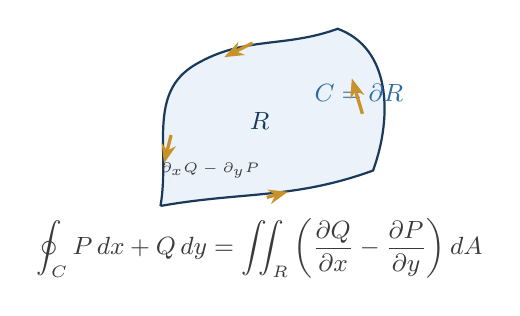
\begin{tikzpicture}
\begin{scope}[scale=0.9]
% Region R with boundary arrows
\draw[NavyBlue,thick,fill=LightBlue] (0,0) to[out=10,in=200] (3,0.5) to[out=70,in=340] (2.5,2.5) to[out=200,in=30] (0.5,2) to[out=210,in=80] (0,0);
\node[NavyBlue,font=\small] at (1.4,1.2) {$R$};
\node[MidBlue,font=\small] at (2.8,1.6) {$C=\partial R$};
% Boundary arrows (CCW)
\draw[-{Stealth[length=7pt]},Gold,very thick] (1.5,0.12) -- (1.8,0.2);
\draw[-{Stealth[length=7pt]},Gold,very thick] (2.85,1.3) -- (2.7,1.8);
\draw[-{Stealth[length=7pt]},Gold,very thick] (1.3,2.3) -- (0.9,2.1);
\draw[-{Stealth[length=7pt]},Gold,very thick] (0.15,1.0) -- (0.05,0.6);
% div/curl inside
\node[DarkGrey,font=\tiny] at (0.7,0.5) {$\partial_xQ-\partial_yP$};
% Label
\node[DarkGrey,font=\small] at (1.4,-0.6) {$\displaystyle\oint_C P\,dx+Q\,dy = \iint_R\left(\frac{\partial Q}{\partial x}-\frac{\partial P}{\partial y}\right)dA$};
\end{scope}
\end{tikzpicture}
\end{center}

\subsection{Step 2: The Divergence Theorem (Gauss)}

\begin{problem}
\label{prob:gauss}
\textbf{Divergence theorem}: for a region $V\subset\mathbb{R}^3$ with outward-oriented boundary $S=\partial V$,
\[
  \iint_S\mathbf{F}\cdot d\mathbf{A} = \iiint_V(\nabla\cdot\mathbf{F})\,dV.
\]
\begin{enumerate}[label=(\alph*),topsep=2pt]
  \item Sketch a proof for a rectangular box $[a_1,b_1]\times[a_2,b_2]\times[a_3,b_3]$ by showing each component of $\nabla\cdot\mathbf{F}$ contributes the flux through the corresponding pair of faces.
  \item Compute the outward flux of $\mathbf{F}=(x^3,y^3,z^3)$ through the sphere $x^2+y^2+z^2=R^2$. Use the divergence theorem and spherical coordinates for the volume integral.
  \item Gauss's law in electrostatics: $\nabla\cdot\mathbf{E} = \rho/\varepsilon_0$. By the divergence theorem, $\iint_S\mathbf{E}\cdot d\mathbf{A} = Q_{\text{enc}}/\varepsilon_0$ where $Q_{\text{enc}}$ is the total charge inside $S$. Use this to find $\mathbf{E}$ outside a uniformly charged sphere of radius $R$ and total charge $Q$ (by choosing $S$ to be a concentric sphere of radius $r>R$).
  \item Derive the continuity equation $\frac{\partial\rho}{\partial t}+\nabla\cdot\mathbf{J}=0$ (conservation of charge/mass/fluid) by applying the divergence theorem to the rate of change of total charge inside a volume.
  \item The divergence theorem reduces a hard surface integral to an easier volume integral (or vice versa). Restate the puzzle calculation using this principle: why was the triple integral easier than the six surface integrals?
\end{enumerate}
\end{problem}

\begin{thought}
\textbf{Conservation laws are divergence theorems.}
The continuity equation $\partial_t\rho + \nabla\cdot\mathbf{J}=0$ says: the rate of change of charge density plus the divergence of current density is zero. This is conservation of charge, derived from the divergence theorem. The same structure gives conservation of mass (in fluid mechanics), conservation of energy (in thermodynamics), and conservation of probability (in quantum mechanics, the probability current). All conservation laws in physics are instances of the same mathematical statement: what flows out of a region equals what is lost inside. The divergence theorem is the mathematical backbone of all conservation.
\end{thought}

\subsection{Step 3: Stokes' theorem}

\begin{problem}
\label{prob:stokes}
\textbf{Stokes' theorem}: for an oriented surface $S$ with boundary curve $C=\partial S$ (orientation consistent),
\[
  \oint_C\mathbf{F}\cdot d\mathbf{r} = \iint_S(\nabla\times\mathbf{F})\cdot d\mathbf{A}.
\]
\begin{enumerate}[label=(\alph*),topsep=2pt]
  \item Show Green's theorem is the special case of Stokes' theorem where $S$ is a flat region in the $xy$-plane.
  \item Use Stokes' theorem to evaluate $\oint_C\mathbf{F}\cdot d\mathbf{r}$ where $\mathbf{F}=(y^2,z,x)$ and $C$ is the boundary of the triangle with vertices $(1,0,0)$, $(0,1,0)$, $(0,0,1)$ oriented counterclockwise when viewed from above.
  \item Show: if $\nabla\times\mathbf{F}=\mathbf{0}$ everywhere (irrotational), then $\oint_C\mathbf{F}\cdot d\mathbf{r}=0$ for any contractible loop. (This is why irrotational fields are conservative on simply connected domains.)
  \item Faraday's law: $\oint_C\mathbf{E}\cdot d\mathbf{r} = -\frac{d}{dt}\iint_S\mathbf{B}\cdot d\mathbf{A}$. By Stokes' theorem, this becomes the differential form $\nabla\times\mathbf{E} = -\partial_t\mathbf{B}$. Show this derivation explicitly. This is one of Maxwell's equations.
  \item Amp\`{e}re's law (with displacement current): $\oint_C\mathbf{B}\cdot d\mathbf{r} = \mu_0\left(I_{\text{enc}} + \varepsilon_0\frac{d\Phi_E}{dt}\right)$. Write the differential form and identify it as another of Maxwell's equations.
\end{enumerate}
\end{problem}

\begin{problem}
\label{prob:maxwell_integral}
\textbf{Maxwell's equations in integral form.} All four Maxwell equations follow from two vector calculus theorems:
\begin{align*}
  \iint_S\mathbf{E}\cdot d\mathbf{A} &= \frac{Q_{\text{enc}}}{\varepsilon_0} \tag{Gauss -- electric}\\
  \iint_S\mathbf{B}\cdot d\mathbf{A} &= 0 \tag{Gauss -- magnetic}\\
  \oint_C\mathbf{E}\cdot d\mathbf{r} &= -\frac{d\Phi_B}{dt} \tag{Faraday}\\
  \oint_C\mathbf{B}\cdot d\mathbf{r} &= \mu_0 I_{\text{enc}} + \mu_0\varepsilon_0\frac{d\Phi_E}{dt} \tag{Amp\`{e}re-Maxwell}
\end{align*}
\begin{enumerate}[label=(\alph*),topsep=2pt]
  \item Convert each to its differential (local) form using Gauss's and Stokes' theorems.
  \item The two Gauss equations use the divergence theorem; the two Faraday/Amp\`{e}re equations use Stokes' theorem. Group them accordingly.
  \item In vacuum ($\rho=0$, $\mathbf{J}=\mathbf{0}$), derive the wave equations for $\mathbf{E}$ and $\mathbf{B}$ using $\nabla\times(\nabla\times\mathbf{E}) = \nabla(\nabla\cdot\mathbf{E}) - \nabla^2\mathbf{E}$. (You derived this in Journey~2 Module~6 deep problem.)
  \item Identify the wave speed and compute $c = 1/\sqrt{\mu_0\varepsilon_0}$. Using $\mu_0 = 4\pi\times10^{-7}$ T$\cdot$m/A and $\varepsilon_0 = 8.85\times10^{-12}$ F/m, verify $c \approx 3\times10^8$ m/s.
  \item Maxwell's 1865 derivation: he had never measured light speed but knew $\mu_0$ and $\varepsilon_0$ from independent electrical measurements. Write two sentences on what it means for a mathematical derivation to predict something that was not being sought.
\end{enumerate}
\end{problem}

\subsection{Step 4: Applications and the unified view}

\begin{problem}
\label{prob:applications}
\begin{enumerate}[label=(\alph*),topsep=2pt]
  \item \textbf{Archimedes' principle via the divergence theorem.} An object submerged in a fluid of density $\rho$ experiences a pressure force $d\mathbf{F} = -\rho g z\,\hat{\mathbf{n}}\,dA$ on each surface element. Show the total buoyancy force is $\mathbf{F}_b = \rho g V\hat{\mathbf{k}}$ where $V$ is the object's volume. \textit{Use the divergence theorem with $\mathbf{G}=(0,0,-\rho gz)$ and compute $\iint_S\mathbf{G}\cdot\hat{\mathbf{n}}\,dA$.}
  \item \textbf{Stokes' theorem and fluid vorticity.} The \textbf{vorticity} of a fluid is $\boldsymbol{\omega}=\nabla\times\mathbf{v}$. The \textbf{circulation} around a closed loop is $\Gamma=\oint_C\mathbf{v}\cdot d\mathbf{r}$. By Stokes' theorem, $\Gamma = \iint_S\boldsymbol{\omega}\cdot d\mathbf{A}$. Interpret: what does it mean for a fluid to have nonzero vorticity?
  \item \textbf{Heat flow.} The heat flux is $\mathbf{q} = -k\nabla T$ (Fourier's law). By the divergence theorem, the rate of heat flowing out of a volume $V$ is $\iint_{\partial V}\mathbf{q}\cdot d\mathbf{A} = -k\iiint_V\nabla^2 T\,dV$. If the total heat energy in $V$ is $\rho c\iiint_V T\,dV$, derive the heat equation $\partial_t T = \kappa\nabla^2 T$ where $\kappa=k/(\rho c)$.
  \item \textbf{Newton's law of gravitation via Gauss.} The gravitational field satisfies $\nabla\cdot\mathbf{g} = -4\pi G\rho$. For a spherically symmetric mass distribution, use Gauss's theorem to derive $\mathbf{g} = -\frac{GM}{r^2}\hat{\mathbf{r}}$ outside the mass.
\end{enumerate}
\end{problem}

\begin{problem}
\label{prob:unified}
\textbf{The generalised Stokes theorem.}

In the language of differential forms from Journey~2, the three theorems are all instances of:
\[
  \int_{\partial\Omega}\omega = \int_\Omega d\omega.
\]
\begin{enumerate}[label=(\alph*),topsep=2pt]
  \item FTC: $\Omega=[a,b]$, $\partial\Omega=\{b\}-\{a\}$, $\omega=f$, $d\omega=f'\,dx$. Verify this gives $\int_a^b f'\,dx = f(b)-f(a)$.
  \item Green's theorem: $\Omega=R\subset\mathbb{R}^2$, $\omega=P\,dx+Q\,dy$ (a 1-form), $d\omega=(\partial_xQ-\partial_yP)\,dx\wedge dy$ (a 2-form). Identify.
  \item Stokes' theorem: $\Omega=S$ (a surface), $\omega=\mathbf{F}\cdot d\mathbf{r}$ (a 1-form), $d\omega=(\nabla\times\mathbf{F})\cdot d\mathbf{A}$. Identify.
  \item Divergence theorem: $\Omega=V$ (a 3D volume), $\omega=\mathbf{F}\cdot d\mathbf{A}$ (a 2-form), $d\omega=(\nabla\cdot\mathbf{F})\,dV$. Identify.
  \item State in one sentence the single principle that unifies the FTC, Green, Stokes, and Gauss: what does every theorem say about the relationship between $\Omega$ and $\partial\Omega$?
\end{enumerate}
\end{problem}

\section{Part 3 \texorpdfstring{---}{--} Discovery}

\begin{discoverybox}
\textbf{What have we built?}

\textbf{First.} Green's theorem (2D), Stokes' theorem (surfaces), and the divergence theorem (3D volumes) are three instances of one principle: the integral of a derivative over a region equals the integral of the original over the boundary.

\textbf{Second.} Each theorem converts between two types of integral (one dimension lower). This is computationally powerful: a hard integral over a surface becomes an easier integral over a volume, or vice versa.

\textbf{Third.} The physical content is immense. Conservation laws (mass, charge, energy, probability) are all instances of the divergence theorem. Faraday's and Amp\`{e}re's laws are instances of Stokes' theorem. Maxwell's equations in integral form are four applications of these two theorems.

\textbf{Fourth.} The unified picture is the generalised Stokes theorem $\int_{\partial\Omega}\omega=\int_\Omega d\omega$. The boundary operator $\partial$ and the exterior derivative $d$ are adjoint to each other in the inner product sense. The identities $\nabla\times\nabla f=\mathbf{0}$ and $\nabla\cdot(\nabla\times\mathbf{F})=\mathbf{0}$ are both instances of $d^2=0$.

\medskip
\textbf{The deep structure.} The complex $f\xrightarrow{d}\omega\xrightarrow{d}\eta\xrightarrow{d}\cdots$ is exact on contractible domains (every closed form is exact) but has non-trivial cohomology on domains with holes. This is topology entering physics: the Aharonov-Bohm effect and Dirac monopoles are consequences of non-trivial topology of the domain.
\end{discoverybox}

\section{Part 4 \texorpdfstring{---}{--} Naming the Ideas}

\begin{namebox}
\textbf{The three integral theorems.}

\textbf{Green's theorem} (2D): $\oint_{\partial R}P\,dx+Q\,dy = \iint_R\left(\frac{\partial Q}{\partial x}-\frac{\partial P}{\partial y}\right)dA$

\textbf{Stokes' theorem} (surface): $\oint_{\partial S}\mathbf{F}\cdot d\mathbf{r} = \iint_S(\nabla\times\mathbf{F})\cdot d\mathbf{A}$

\textbf{Divergence theorem} (volume): $\iint_{\partial V}\mathbf{F}\cdot d\mathbf{A} = \iiint_V(\nabla\cdot\mathbf{F})\,dV$

\textbf{Master theorem}: $\int_{\partial\Omega}\omega = \int_\Omega d\omega$ (all three are special cases, as is the FTC).
\end{namebox}

\section{Part 5 \texorpdfstring{---}{--} Deep Problems}

\begin{deepproblem}[Proof of Stokes' theorem via Green's theorem]
\begin{enumerate}[label=(\alph*)]
  \item Parametrise the surface $S$ by $\mathbf{r}(u,v)$ with $(u,v)\in D\subset\mathbb{R}^2$. Write $\oint_{\partial S}\mathbf{F}\cdot d\mathbf{r}$ as a line integral over $\partial D$.
  \item Apply Green's theorem on $D$ to convert the line integral over $\partial D$ to a double integral over $D$.
  \item Show the resulting double integral equals $\iint_S(\nabla\times\mathbf{F})\cdot d\mathbf{A}$ by expanding $((\nabla\times\mathbf{F})\cdot(\mathbf{r}_u\times\mathbf{r}_v))$ and using the chain rule. (This is a substantial computation: work one component at a time.)
  \item The proof works for any parametrisation. Show the final answer is independent of the choice of parametrisation, as it must be (the left side $\oint_{\partial S}\mathbf{F}\cdot d\mathbf{r}$ is defined independently of parametrisation).
\end{enumerate}
\end{deepproblem}

\begin{deepproblem}[de Rham cohomology via the integral theorems]
\begin{enumerate}[label=(\alph*)]
  \item A \textbf{closed} $k$-form satisfies $d\omega=0$; an \textbf{exact} form satisfies $\omega=d\eta$. Every exact form is closed. The de Rham cohomology $H^k(M)$ measures the failure of the converse.
  \item Compute $H^1(\mathbb{R}^2)$: show every closed 1-form on $\mathbb{R}^2$ is exact. (If $dP=dQ$, construct $f(x,y)=\int_0^x P(t,0)\,dt+\int_0^y Q(x,t)\,dt$ and verify $df=Pdx+Qdy$.)
  \item Compute $H^1(\mathbb{R}^2\setminus\{0\})=\mathbb{R}$: show the form $\omega=\frac{-y\,dx+x\,dy}{x^2+y^2}$ is closed but not exact, and that every closed 1-form on $\mathbb{R}^2\setminus\{0\}$ is $c\omega+df$ for some constant $c$ and function $f$.
  \item For a torus $T^2=S^1\times S^1$: state (without proof) $H^0(T^2)=\mathbb{R}$, $H^1(T^2)=\mathbb{R}^2$, $H^2(T^2)=\mathbb{R}$. Interpret $H^1(T^2)=\mathbb{R}^2$: there are two independent non-contractible loops on the torus. What are they?
  \item \textbf{Physical meaning.} In electromagnetism on a non-simply-connected domain (e.g.\ a toroidal solenoid), $H^1\neq 0$ implies that there can be $\nabla\times\mathbf{A}\neq\mathbf{0}$ (magnetic flux) even though $\mathbf{A}$ is not globally well-defined. This is precisely the Aharonov-Bohm effect. Write two sentences connecting de Rham cohomology to observable physics.
\end{enumerate}
\end{deepproblem}

\begin{deepproblem}[Differential forms in $n$ dimensions]
\begin{enumerate}[label=(\alph*)]
  \item A $k$-form on $\mathbb{R}^n$ is a totally antisymmetric multilinear map from $k$ tangent vectors to $\mathbb{R}$. The space of $k$-forms at a point has dimension $\binom{n}{k}$. Verify: in $\mathbb{R}^3$, there are $\binom{3}{0}=1$ scalar fields (0-forms), $\binom{3}{1}=3$ components of 1-forms, $\binom{3}{2}=3$ components of 2-forms, $\binom{3}{3}=1$ scalar field (3-form).
  \item The exterior derivative $d$ maps $k$-forms to $(k+1)$-forms and satisfies $d^2=0$. Show $d$ applied to a 0-form (scalar) gives the gradient; to a 1-form in $\mathbb{R}^3$ gives the curl; to a 2-form in $\mathbb{R}^3$ gives the divergence. This shows grad, curl, div are all the same operation!
  \item The \textbf{Hodge star} $\star$ maps $k$-forms to $(n-k)$-forms using the inner product and orientation. In $\mathbb{R}^3$: $\star(dx)=dy\wedge dz$, etc. Show $\star d$ applied to a 1-form gives $\nabla\times$ (curl), and $\star d\star$ applied to a 1-form gives $-\nabla\cdot$ (negative divergence).
  \item The \textbf{Laplace-de Rham operator} $\Delta = d\delta+\delta d$ (where $\delta=(-1)^k\star d\star$) generalises the scalar Laplacian to $k$-forms. A \textbf{harmonic form} satisfies $\Delta\omega=0$. On a compact manifold, $H^k(M)\cong\ker\Delta_k$ (the Hodge decomposition). State what this says about the relationship between topology and analysis.
\end{enumerate}
\end{deepproblem}

\section{Part 6 \texorpdfstring{---}{--} Reflection}

\begin{reflectionbox}
\textbf{Your reflection task.}

\begin{enumerate}
  \item \textbf{On Maxwell's equations.} Maxwell derived the speed of light from equations governing electricity and magnetism, two phenomena that had seemed entirely separate. He unified them. Write a paragraph: what does unification mean in physics? Is it about finding that two things are the same, or finding that they are special cases of something more general?

  \item \textbf{On the boundary.} All three theorems say: what happens inside is determined by what happens on the boundary. This principle appears throughout mathematics (harmonic functions are determined by boundary values, topological invariants come from boundary maps, quantum amplitudes depend on boundary states). Does this principle feel deep to you, or accidental?

  \item \textbf{On $d^2=0$.} The identities $\nabla\times(\nabla f)=0$ and $\nabla\cdot(\nabla\times\mathbf{F})=0$ both follow from $d^2=0$. This single algebraic identity underlies both physical facts (curl of a gradient is zero, divergence of a curl is zero) and topological measurement (de Rham cohomology counts holes). Write one sentence on how an algebraic rule generates both physical and topological content.

  \item \textbf{Looking ahead.} Module~3 studies the Laplacian and the equations of classical physics: Laplace's equation, the wave equation, and the heat equation. You now have all the tools to derive them from first principles. Before reading further: write the Laplace equation, wave equation, and heat equation, and state which physical systems each describes.
\end{enumerate}
\end{reflectionbox}

\medskip
\noindent\textbf{Looking ahead.}
Module~3 studies the three great PDEs of classical physics: Laplace's equation (electrostatics, gravitation, steady-state heat), the wave equation (sound, light, water), and the heat equation (diffusion, probability). All three involve the Laplacian. All three are solved by separation of variables, producing eigenvalue problems and Fourier series.

\vspace{1.4cm}
\begin{center}
{\color{MidBlue}\rule{0.5\linewidth}{0.8pt}}\\[6pt]
{\small\color{DarkGrey}\textit{End of Journey 4, Module 2 --- The Integral Theorems}}\\[4pt]
{\small\color{DarkGrey}Continue to: \textbf{Module 3 --- The Classical PDEs}}\\[6pt]
{\color{MidBlue}\rule{0.5\linewidth}{0.8pt}}
\end{center}

\end{document}